\section{Experiment}
\label{sec:exp}

In this section, we will describe how we set up 
experiments to evaluate \Tool{} (Section~\ref{sec:meth}) 
and present the experimental results (Section~\ref{sec:results}). 

\subsection{Methodology}
\label{sec:meth}

\noindent\textbf{Implementation and Platform.} 
We implement \Tool{} using LLVM-7.0.0~\cite{LLVM}, 
and conduct our experiments on a Linux machine, 
with E5-2630 CPU, 32GB memory and 3.10 kernel. 

\noindent\textbf{Benchmarks.}
\Tool{} is a tool to automatically extract FSMs implemented in a program. 
Since we build \Tool{} using LLVM, 
our current implementation can only work on C/C++ programs.  
However, we believe that our algorithm is general enough 
to be extended to other programming languages. 


To evaluate \Tool{}, we collect C/C++ programs from three sources. 
First, we evaluate \Tool{} on two programs collected in a CTF contest~\cite{ctf}, 
one contains a FSM, and the other one does not. 
Second, we leverage the DARPA CGC dataset~\cite{CGC}. 
In total, there are 197 programs in the CGC dataset.
As discussed in Section~\ref{sec:study}, 
we already use 40 of them to conduct our empirical study,
so that we use the remaining 157 programs in our evaluation.
Third, we apply \Tool{} to OpenVPN~\cite{openvpn}, 
which provides an implementation of virtual private network and 
is included in software packages of every released Linux version. 

\vspace{-0.1in}
\begin{table}[h!]
\centering
\footnotesize
%\scriptsize

 %\setlength{\tabcolsep}{0.8mm}{
 \setlength{\tabcolsep}{1.6mm}{
\begin{tabular}{|l|c|c|c|c|}
\hline
\textbf{Source}   & \textbf{\# programs} & \textbf{avg. KLOC} & \textbf{\# loops} & \textbf{\# FSM loops} \\ \hline \hline 
CTF     & 2              &  0.3            &    19       &   1         \\ \hline 
CGC     & 157            &  7.1            &    6607     &   59        \\ \hline
OpenVPN & 1              &  120            &    512      &    6        \\ \hline
\end{tabular}
}
%\vspace{0.1in}
\vspace{0.1in}
\mycaption{tab:benchmark}
{Benchmark Information.}
{}
%{KLOC: thousand lines of code. }
%  \label{tab:apps}
\vspace{-0.15in}
\end{table}

The benchmark information is shown in Table~\ref{tab:benchmark}.
In total, we use 160 different programs to evaluate \Tool{}.
Our benchmark set is a representative sample of real-world software, 
since each program is either a widely-used real application or a simplified program
from real software. 
Our benchmark programs are diverse. 
They cover programs in small, medium and large sizes, 
with lines of code ranging from 0.3 thousand to more than 100 thousand.  
There are more than seven thousand 
loops inside our benchmark programs and accurately 
identifying FSMs among the loops is not easy. 
To sum up, we believe that our benchmarks are good 
enough to evaluate the effectiveness of \Tool{}.

\noindent\textbf{Evaluation Setting.} 
For all our benchmark programs, we manually examine all their loops and 
identify all FSM loops. 
As shown in Table~\ref{tab:benchmark}, there are in 
total 66 FSM loops.
Four FSM loops contain two state variables, 
and all other FMS loops contain exact one state variables.
Therefore, there are in total 70 FSMs implemented in all our benchmarks.  
We apply \Tool{} to all benchmark programs. 
We mainly compute metrics to answer two research 
questions regarding the coverage and accuracy of \Tool{}.

\textbf{Q1. Coverage:} whether \Tool{} can identify all implemented FSMs?
 
\textbf{Q2. Accuracy:} whether \Tool{} will report loops, which are FSM loops, 
generating false positives. 

\subsection{Experimental Results}
\label{sec:results}

\begin{table}[h!]
\centering
\footnotesize
\setlength{\tabcolsep}{1.6mm}{
\begin{tabular}{|l|c|c|c|c|}
\hline
\textbf{Source}   & \textbf{\# FSM loops} & \textbf{\# FSMs} & \textbf{\# FNs} & \textbf{\# FPs} \\ \hline \hline 
CTF               &   1                   &  1              & 0    & 0       \\ \hline 
CGC               &   59                  &  63             & 0    & 2        \\ \hline
OpenVPN           &   6                   &  6              & 0    & 0         \\ \hline
\end{tabular}
}

\mycaption{tab:exp}
{Experimental Results.}
{}
%{FN: false negative, and FP: false positive.}
\vspace{0.1in}
\end{table}

\noindent\textbf{Coverage.}
As shown in Table~\ref{tab:exp}, \Tool{} successfully identifies 
all the 66 FSM loops 
from the benchmarks. Since there are four FSM loops containing 
two state variables and \Tool{} constructs a FSM for every identified state variable, 
there are in total 70 extracted FSMs. 
\Tool{} has \textbf{no} false negative.

We then further inspect the characteristics of the identified FSMs.
For most of the FSMs, their state variables are local variables.
There are only three FSMs with a global variable as its state variable. 
Most FSMs use a standalone integer (or enumeration) variable as its state variable,
and only three FSMs use a \texttt{struct} field as its state variable.  
This result shows that \Tool{} can identify state variables implemented in various ways
and developers tend to use a local, standalone, integer variable to 
represent the state of a FSM.


{
\begin{figure}[t]
\begin{minipage}{\columnwidth}
\begin{center}
\centerline{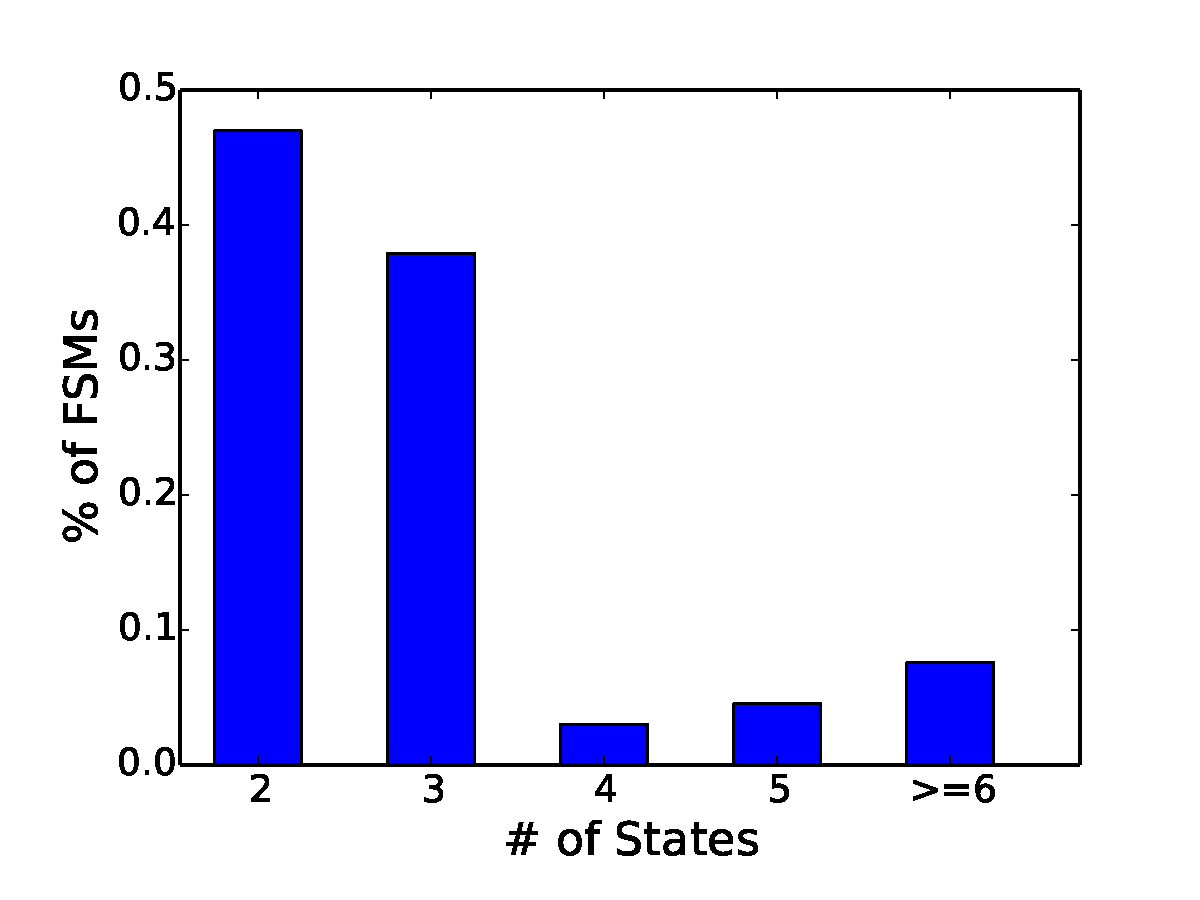
\includegraphics[width=2.5in]{figure/sv-dist.pdf}}
%\vspace{-0.05in}
\mycaption{fig:sv}{How the number of states distributes across all identified FSMs.}
{}
\end{center}
\end{minipage}
%\vspace{0.1in}
\end{figure}
}

Figure~\ref{fig:sv} shows the percentage of the identified FSMs
for different state numbers. 
More than 80\% of FSMs contain either two states or three states. 
The percentage drops significantly when the state number is larger than three. 
There are two FSMs containing 11 states. 
These two FSMs have the largest state numbers among all the identified FSMs. 
On average, one identified FSM has 3.02 possible states. 
Figure~\ref{fig:sv} also shows how the percentage of FSMs distributes 
across different state numbers 
for the 25 studied FSMs. 
The average state number for the studied FSMs is 3.84.
We use chi-square goodness of fit test to compare 
the two distribution in Figure~\ref{fig:sv}. 
The testing result shows that there is no significant 
difference between the two distributions 
under 99\% confidence level. 
Our study results in Section~\ref{sec:study} are general enough to be 
extended to other data sets. 




\noindent\textbf{Accuracy.}
\Tool{} reports two false positives when analyzing CGC programs. 
One of the example is shown in Figure~\ref{XXX}


\subsection{Case Study}